\documentclass[12pt]{article}
\usepackage{amsmath}
\usepackage{amsfonts}
\usepackage{geometry}
\usepackage{graphicx}
\usepackage{setspace}
\usepackage{parskip}
\usepackage{hyperref}
\usepackage{graphicx}
\usepackage{float}
\newcommand{\comm}[1]{def}

\geometry{a4paper, margin=1in}
\setstretch{1.2}

\title{\Huge Orderbook Delta price reaction research}
\author{}
\date{}





    


\begin{document}

\maketitle


\subsection*{Table of Contents}

\begin{itemize}
  \item Outlier Detection Using Mean and Standard Deviation (Z-Score Based Outlier Detection)
  \item Measuring Volatility After Price Outlier Detection
  \item Measuring avearge return after price outlier detection
  \item Combining Indicators
\end{itemize}


\newpage

\section*{Outlier Detection Using Mean and Standard Deviation (Z-Score Based Outlier Detection)}


\subsection*{Normal Range}

What I want to test is how price reacts to anomalous orderbook delta movements, particularly in scenarios where unrealistic or clearly outlying values are detected. In cryptocurrency markets, such inefficiencies can be caused by various events, one example is liquidation
 events that interact with passive demand order stacked zones. During these events, the orderbook delta exhibits significant increases, providing a clear signal of market stress. This research will focus on understanding the relationship between rapid delta movements and how price reacts after these events.

\subsection*{My Hypothesis}

\begin{itemize}
  \item I expext realized volatility to increase after an outlier is detected. 
  \item I expext a return to the mean after a strong outlier is detected.
\end{itemize}



\subsection*{Normal Range}





\[
\mu(\Delta) \pm 2\sigma(\Delta)
\]

This means most data points (about 95\% if normally distributed) are expected to lie within this range.

\newpage

\subsection*{Outlier Condition}

A value is considered an outlier if:



\begin{equation}\label{eq: outlier_detection}
  \Delta < \mu(\Delta) - 2\sigma(\Delta) \quad \text{or} \quad \Delta > \mu(\Delta) + 2\sigma(\Delta)    
\end{equation}

This is a simple Z-score based outlier detection.

\begin{itemize}
  \item $\Delta$ - Orderbook Delta Depth with a certain depth I will test on: $\Delta_{1\%}$ $\Delta_{2.5\%}$ $\Delta_{5\%}$ from Coinbase (BTC/USD) 
  \item   This basically means we take a delta of the Bid and Ask orders which are in a range of x\% from the current price.
  \item $\mu(\Delta)$ — Mean of the last 1440 values of $\Delta$ before time $t$
  \item $\sigma(\Delta)$ - Standard deviation over the last 1440 $\Delta$ values before time $t$

\end{itemize}










\newpage


\subsection*{Idea behind}

\begin{itemize}
    \item This method assumes data is roughly normally distributed.
    \item Using $2\sigma$ captures approximately 95\% of data points under a normal distribution.
    \item You can adjust the multiplier (e.g., $3\sigma$) for stricter or looser thresholds.
\end{itemize}





\subsection*{Future Plans}

\begin{itemize}
    \item Test on more data
    \item use rolling windows (e.g. 1 day or 1 week) for local context.
    \item Compare sensitivity with +- 1.5$\sigma$ or +-2.5$\sigma$ $\rightarrow$ optimize for best results
\end{itemize}
















\newpage





\section*{Measuring Volatility After Price Outlier Detection}


\begin{equation}\label{eq:price_return}
    r_t = \frac{P_{t} - P_{t-1}}{P_{t-1}}
\end{equation}


\subsection*{Dictionary of Terms}

\begin{itemize}
    \item $P_t$  
      Asset price at time $t$.
    \item $r_t = \dfrac{P_t - P_{t-1}}{P_{t-1}}$  
      – 1-minute price return at time $t$.
    \item $\sigma^{\mathrm{(15)}}_{t}$  
      – Realized volatility: the standard deviation of the next 15 one-minute returns,
      
      

      
      \begin{equation}\label{eq:realized-vol}
        \sigma^{\mathrm{(15)}}_{t}
        = \sqrt{\frac{1}{14}\sum_{i=1}^{15}\bigl(r_{t+i}-\bar r_{t}\bigr)^{2}},
        \quad
        \bar r_{t} = \frac{1}{15}\sum_{i=1}^{15} r_{t+i}.
      \end{equation}
      



      aligned so that at time $t$ it measures volatility over $t+1$ to $t+15$.
\end{itemize}



\subsection*{In Py code}

\begin{verbatim}
import pandas as pd
df = pd.read_csv(file_path)
df.set_index('timestamp', inplace=True)
#Compute 1-min return of delta_5

df['r_t'] = df['price'].pct_change().fillna(0)


#compute rolling std of the future 15 min window

window = 15

#rolling on r_t, then shift forward so index t hold vol of t+1...t+15
df['future_vol_15] = (
    df['r_t']
    .rolling(window=window)
    .std()
    .shift(-window)
)
\end{verbatim}



\newpage

\subsection*{\textbf{Statistical evidence}}

Once an outlier is detected \eqref{eq: outlier_detection} inside of the Orderbook $\Delta$, we calculate the15-minute ahead realized volatility using Equation: \eqref{eq:realized-vol}




if a $\Delta_t$ values is flagged as an outlier \eqref{eq: outlier_detection}
we record
$$
\sigma^{(15)}_t
\;=\;
\sqrt{\frac{1}{14}\sum_{i=1}^{15}\bigl(r_{t+i}-\bar r_{t}\bigr)^{2}},
$$

We then form two samples over our full dataset which during this test includes 104 957 one minutes intervals of $P$ and Orderbook $\Delta$:


$$
\mathcal{S}_{\rm out} \;=\;\{\sigma^{(15)}_t : t\text{ is an outlier}\},
\quad
\mathcal{S}_{\rm non} \;=\;\{\sigma^{(15)}_t : t\text{ is not an outlier}\}.
$$


Sample mean results:
$$
\overline{\sigma}^{(15)}_{\rm out}
=0.0006244,
\qquad
\overline{\sigma}^{(15)}_{\rm non}
=0.0005138,
$$




This concludes an increase of $r_t$ of roughly 21.5\%


To check Statistical evidence

\begin{itemize}
  \item a two-sample *t*-test (unequal variances), which yields
  $$
    T=24.72,\quad p=4.79\times10^{-132},
  $$
  \item a Mann–Whitney *U*-test, which returns
  $$
    p=4.02\times10^{-157}.
  $$
\end{itemize}


\newpage

\section*{Opmtimings for best Z-Score thresold for outliers}

As state inside of \eqref{eq: outlier_detection} we use a Z-Score thresold of 2 to detect outliers. I now want to 
see if by any chance there is a better Thresold value  








\newpage
\section*{Measuring avearge return after price outlier detection}




\subsection*{Formulars}
\begin{align}
\intertext{Once a $\Delta_t$ Outlier is detected we calculate the 15-min forward return of \underline{BTC/USD} price}
\mathrm{Ret}^{(15)}_t
\;=\;\frac{P_{t+15} - P_t}{P_t}
\tag{4}\\[1ex]
\intertext{We then differentiate between a bullish and a bearish outlier. Which is already defined \eqref{eq: outlier_detection}}
\overline{\mathrm{Ret}}^{(15)}_{\rm bull}
= \frac{1}{|\mathcal{T}_{\rm bull}|}
  \sum_{t\in\mathcal{T}_{\rm bull}} \mathrm{Ret}^{(15)}_t
\tag{7}\\[1ex]
\overline{\mathrm{Ret}}^{(15)}_{\rm bear}
= \frac{1}{|\mathcal{T}_{\rm bear}|}
  \sum_{t\in\mathcal{T}_{\rm bear}} \mathrm{Ret}^{(15)}_t
\tag{8}
\end{align}







\subsection*{Dictionary of Terms}

\begin{itemize}
  \item Price at a certain time: \space $P_t$
  \item 15-min forward return: \space $\mathrm{Ret}^{(15)}_t$
\end{itemize}





\begin{verbatim}
  #compute 15-min forward return of BTC/USD price
\end{verbatim}




\newpage

\section*{Combining Indicators}
Here I visulised the swing points, the EMA spread and the 100 outliers with the highest Z-Score in the same plot.

\begin{figure}[H]
    \centering
    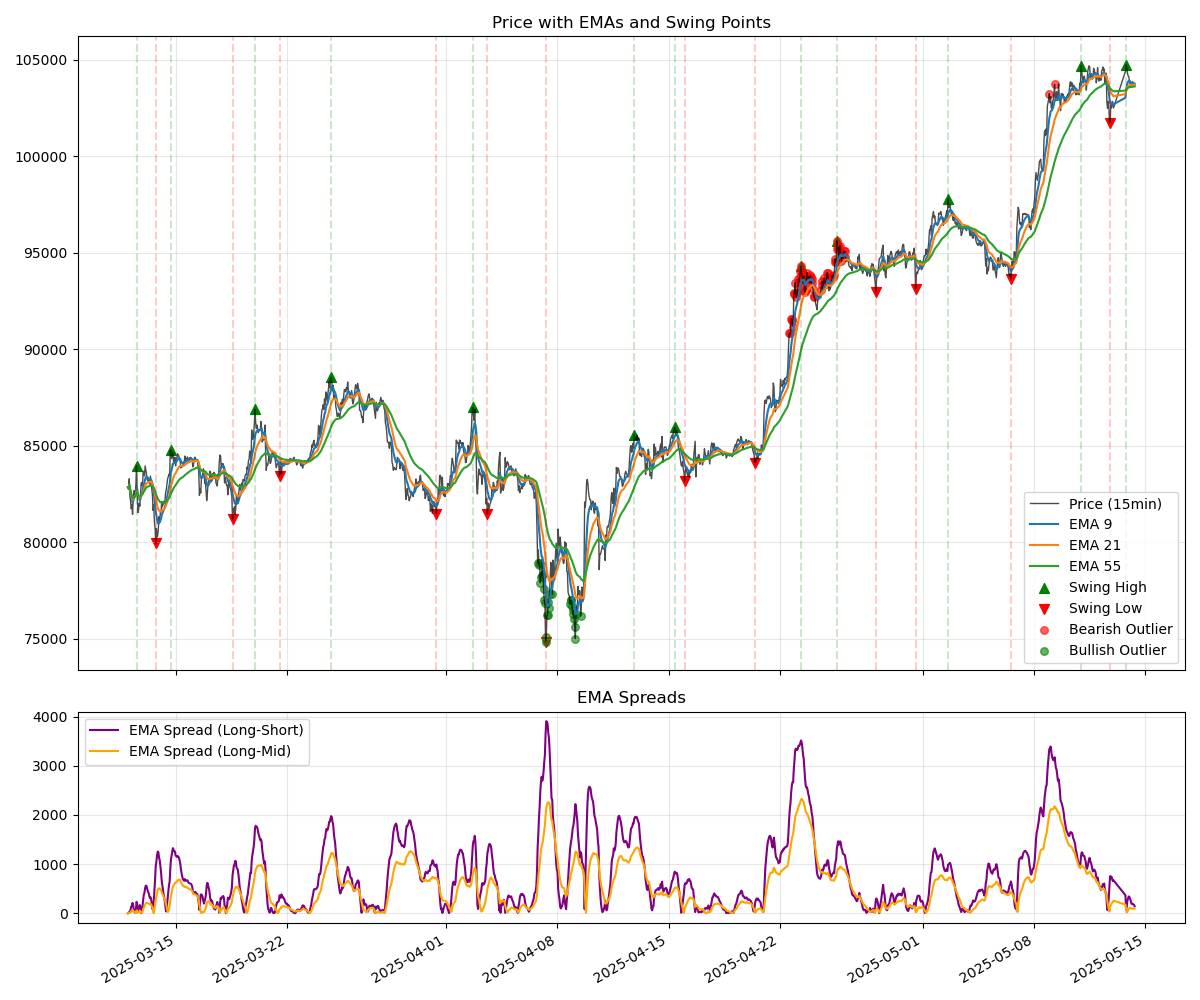
\includegraphics[width=\textwidth]{imgs/swingpoints_emaspread_priceOutliers.png}
    \caption{combined indicators png}
\end{figure}

\footnote{Chart made with Matplotlib and Seaborn}

\end{document}